\chapter{Hidden-State Probing: Setup and Results}
\label{chap:probing-results}

Chapter~\ref{chap:dataset-construction} confirms that the single-turn and multi-turn datasets are suitable for a probing experiment.

This chapter describes the experimental setup and reports the results obtained on eight open-weight models. Section~\ref{sec:model-choice} describes the eight models first, since the routing task, the hidden-state capture, the layer sweep and the results of the later sections are all defined for each model. Section~\ref{sec:ch7-probing-setup} describes the coordinator's routing task, the hidden-state capture procedure, the layer sweep that trains one probe per layer to find the optimal layer, and the metrics used to compare the probe against the model. Section~\ref{sec:ch7-results} reports the results obtained for each model, on the single-turn and the multi-turn dataset. Section~\ref{sec:ch7-observations} summarizes what these results show, including whether the differences between probe and model are significant.


\section{Model Choice}
\label{sec:model-choice}

The experiment runs on eight open-weight models, chosen to satisfy the requirements of Section~\ref{subsec:model-pool-requirements}. The model pool spans:

\begin{itemize}
    \item the Gemma 4 family by Google DeepMind \cite{teamGemma4Technical2026}, at three parameter sizes: E2B (5B total parameters, of which 2.3B are effective due to its internal architecture \cite{teamGemma4Technical2026}), 12B, and 26B A4B (a mixture-of-experts model, as defined in Section~\ref{subsec:dense-moe}, with 26B total parameters, of which 3.8B are active per token \cite{teamGemma4Technical2026}). Gemma 4 is the latest model family that Google DeepMind had released as of this writing (September 2026)
    \item the Qwen3 family by the Qwen Team (Alibaba) \cite{yangQwen3TechnicalReport2025}, at two parameter sizes: 4B and 8B
    \item GPT-OSS 20B by OpenAI \cite{openaiGptoss120bGptoss20bModel2025}
    \item Llama 3.3 70B Instruct by Meta \cite{MetallamaLlama3370BInstructHugging2024}
    \item Qwen2.5 72B Instruct by the Qwen Team (Alibaba) \cite{qwenQwen25TechnicalReport2025}
\end{itemize}

The model pool allows the probe to be tested on models from different providers, whose parameter count spans from a few billion to over seventy billion. Table~\ref{tab:model-properties} reports the architecture, parameter count, and layer count of each model. Each model family also relies on its own chat template, which is needed to format the prompt and the tool definitions correctly and to read the response correctly, as described in Section~\ref{subsec:rendered-example}.

Every model is configured to generate with sampling disabled, under greedy decoding as described in Section~\ref{subsec:decoding}, so that its routing decision is deterministic. This setting satisfies the replicability requirement that Section~\ref{subsec:model-pool-requirements} states for the model pool.

\begin{table}[htbp]
    \centering
    \footnotesize
    \setlength{\tabcolsep}{4pt}
    \begin{tabular}{lllrrrrl}
        \toprule
        Full name & Identifier & Provider & Total & Active & Layers & $d_{\mathrm{model}}$ & Chat template \\
        \midrule
        Gemma 4 E2B IT & \texttt{gemma4-e2b-it} & Google DeepMind & 5B & 2.3B & 35 & 1536 & gemma4 \\
        Qwen3 4B Instruct 2507 & \texttt{qwen3-4b} & Qwen Team (Alibaba) & 4B & 4B & 36 & 2560 & hermes \\
        Qwen3 8B & \texttt{qwen3-8b} & Qwen Team (Alibaba) & 8B & 8B & 36 & 4096 & hermes \\
        Gemma 4 12B IT & \texttt{gemma4-12b-it} & Google DeepMind & 12B & 12B & 48 & 3840 & gemma4 \\
        GPT-OSS 20B & \texttt{gpt-oss-20b} & OpenAI & 20.9B & 3.6B & 24 & 2880 & harmony \\
        Gemma 4 26B A4B IT & \texttt{gemma4-26b-a4b-it} & Google DeepMind & 26B & 3.8B & 30 & 2816 & gemma4 \\
        Llama 3.3 70B Instruct & \texttt{llama3.3-70b} & Meta & 70B & 70B & 80 & 8192 & llama3 \\
        Qwen2.5 72B Instruct & \texttt{qwen2.5-72b} & Qwen Team (Alibaba) & 72B & 72B & 80 & 8192 & hermes \\
        \bottomrule
    \end{tabular}
    \caption[Properties of the eight models used in this chapter]{Properties of the eight models used in this chapter.}
    \label{tab:model-properties}
\end{table}

\subsection{Chain-of-Thought Output}
\label{subsec:ch7-reasoning-traces}

Section~\ref{subsec:chain-of-thought} describes chain-of-thought output as text that a model generates before its response. Both the Gemma 4 family and the Qwen3 family in this pool call this a \emph{thinking mode} and let it be turned on or off at inference time \cite{teamGemma4Technical2026, yangQwen3TechnicalReport2025}.

In this work, thinking mode is always turned off where available, so the models are compared under the same condition. The only exception is GPT-OSS 20B, which, by design, does not allow chain-of-thought output to be disabled \cite{openaiGptoss120bGptoss20bModel2025}. Instead, GPT-OSS 20B exposes a \emph{reasoning effort} setting, with three levels (\texttt{low}, \texttt{medium}, \texttt{high}), that controls how long this chain-of-thought output is \cite{openaiGptoss120bGptoss20bModel2025}. In this work, the reasoning effort is set to \texttt{low}.


\section{Probing Setup and Routing Task}
\label{sec:ch7-probing-setup}

\subsection{Coordinator Setup}
\label{subsec:ch7-coordinator-prompt}

Each model in the pool of Section~\ref{sec:model-choice} is used as the coordinator of the centralized topology described in Section~\ref{subsec:topology-centralized}: a single supervisor that reads one request, single-turn or multi-turn, and routes it to one of the five sub-agents from Section~\ref{subsec:sub-agent-taxonomy}. A system prompt instructs the model on its coordinator role and the routing task that it has to perform, and lists the collision graph of Section~\ref{subsec:collision-graph}. The prompt is shared by all eight models and reported in Appendix~\ref{sec:appendix-coordinator-prompt}.

The coordinator states its routing decision through the function-calling interface described in Section~\ref{sec:structured-output}. Each sub-agent is declared to the model as a tool, and the coordinator routes a request by calling the tool representing the chosen sub-agent exactly once. Each tool's description states the sub-agent's role, the type of concerns that it handles, and an example request that routes to it. Each tool requires no argument from the coordinator. The five tool definitions are reported in Appendix~\ref{sec:appendix-subagent-tools}. The tool declarations are rendered into the prompt alongside the system prompt by the model's own chat template, the same mechanism that Section~\ref{subsec:rendered-example} describes for formatting a prompt and its tool definitions. The model's prediction is therefore obtained by reading which one of the available tools the model invokes.

None of the five sub-agents is implemented: the experiment only records which tool the coordinator invokes.

\subsection{Hidden-State Capture and the Model's Prediction}
\label{subsec:ch7-hook}

For every request, the same run of the model is used to obtain both the hidden states and the tool call that defines the model's own routing decision. This capture follows the fixed sequence of steps shown in Figure~\ref{fig:hook-sequence}.

\begin{figure}[ht]
	\centering
	\vspace{4mm}
	\begin{tikzpicture}[
		node distance=5mm,
		every node/.style={font=\small},
		seqstep/.style={draw, rounded corners, align=left, text width=0.82\textwidth, inner sep=5pt},
		seqcapture/.style={draw, dashed, rounded corners, align=left, text width=0.82\textwidth, inner sep=5pt},
		arr/.style={-{Latex[length=2mm]}}
		]
		\node[seqstep] (s1) {\textbf{Step 1:} the request is submitted to the coordinator.};
		\node[seqstep, below=of s1] (s2) {\textbf{Step 2:} the coordinator processes the request in the prefill step, described in Section~\ref{subsec:prefill-decode}, with no response token generated yet.};
		\node[seqcapture, below=of s2] (s3) {%
			\begin{minipage}{\linewidth}
				\textbf{Step 3:} the hidden states for every layer $\ell$ are read at the last prompt token $n$, by a forward hook registered on every layer through the PyTorch \texttt{nn.Module} API \cite{ModulePyTorch214}.
				\begin{center}
					\vspace{2pt}
					$h^{(\ell)}_n, \quad \forall \ell = 1, \dots, L$
					\vspace{2pt}
				\end{center}
				where $h^{(\ell)}_n$ is the hidden-state vector of layer $\ell$ at the last prompt token $n$, as defined in Section~\ref{subsec:hidden-states}.
			\end{minipage}
		};
		\node[seqstep, below=of s3] (s4) {\textbf{Step 4:} generation proceeds, one token at a time, until termination is reached.};
		\node[seqstep, below=of s4] (s5) {\textbf{Step 5:} the tool call in the generated response is parsed with the model's own function-calling syntax. The tool call is recorded as the \textbf{model} prediction.};
		\foreach \x/\y in {s1/s2, s2/s3, s3/s4, s4/s5}
			\draw[arr] (\x) -- (\y);
	\end{tikzpicture}
	\caption[Sequence of steps to capture hidden states and model prediction]{The sequence of steps used to capture the hidden states and the model prediction for one request.}
	\label{fig:hook-sequence}
\end{figure}

Submitting a sample of the single or multi-turn dataset to a model provides two additional features for that sample: the hidden states captured at every layer for the last prompt token, and the model prediction. The hidden states are stored as 16-bit floating-point values. The model prediction is considered correct when it matches \texttt{gold}, the correct sub-agent defined for the sample in Section~\ref{subsec:design-factors}.

\subsection{Probe Training}
\label{subsec:ch7-probe}

For every model and dataset, one \emph{probe} is trained for each layer $\ell$. The probe for layer $\ell$ is trained on the hidden state $h^{(\ell)}_n$ from that same layer, for every sample, to predict the sample's gold sub-agent. This procedure is called a \emph{layer sweep}, and it determines the \emph{optimal layer} $\ell_o$: the layer whose probe reaches the highest accuracy, defined as the fraction of samples for which the probe predicts the correct sub-agent. If more than one layer reaches the highest accuracy, the layer with the lowest index $\ell$, closest to the input, is selected as $\ell_o$.

Each probe is trained as a logistic regression classifier, making it a \emph{linear probe}. Before fitting, each layer's hidden states are standardized to zero mean and unit variance, because they are read before the block's layer normalization is applied, so their scale can vary sharply across dimensions and across models.

A probe is evaluated with the same scenario-grouped 5-fold cross-validation used for the text-only baselines in Section~\ref{subsec:text-only-baselines}: the two near-duplicate queries of an \texttt{adversarial} pair always fall in the same fold, so when one query is held out for testing, its near-duplicate is held out with it, instead of leaking into the training folds.

\subsection{Execution Infrastructure}
\label{subsec:ch7-infra}

The process described in Section~\ref{subsec:ch7-hook} requires GPU compute, since the model must be loaded in memory and every layer's hidden states must be read during the forward pass. Each run submits one dataset to one model and executes on Modal \cite{ModalDocumentation}, a serverless platform that provisions several kinds of GPU containers on demand. One or more parallel NVIDIA H100 and A100 GPUs are used per run, to guarantee sufficient VRAM to load the unquantized model weights and to submit the requests to the model in batches. A linear probe, instead, requires little computation to train and can therefore be trained locally, on consumer hardware.

\subsection{Metrics}
\label{subsec:ch7-metrics}

\paragraph{Accuracy.} Accuracy is the fraction of samples for which a classifier predicts the correct sub-agent. The probe and the text-only classifiers of Section~\ref{subsec:text-only-baselines} follow the same procedure, on the same scenario-grouped 5-fold cross-validation of Section~\ref{subsec:ch7-probe}. Each fold is held out once, the classifier is trained on the other four folds, and its accuracy is measured on the held-out fold. The reported accuracy is the mean of the five fold accuracies, taken at the optimal layer $\ell_o$ for the probe. The model is not trained on the dataset, so its predictions do not depend on the folds. Its accuracy is still measured on each of the five folds and averaged, so the model, the probe and the text-only classifiers are scored on the same samples with the same rule.

\paragraph{AUC macro.} AUC (area under the curve) macro is the area under the ROC (receiver operating characteristic) curve of the probe at the optimal layer $\ell_o$, computed once for each sub-agent on the out-of-fold probabilities and averaged with equal weight across the five sub-agents. AUC macro splits the five-way prediction of the probe into five binary problems. The binary problem of a sub-agent $a$ separates the samples whose correct sub-agent is $a$ from the samples of the other four sub-agents, which is how ROC analysis handles more than two classes \cite{fawcettIntroductionROCAnalysis2006}.

For each sample, the probe assigns a probability to $a$, and the sample is predicted as $a$ when this probability is above a cut-off value $t$, called the \emph{threshold}. For a given $t$, the true positive rate is the fraction of samples of $a$ predicted as $a$, and the false positive rate is the fraction of the other samples predicted as $a$. The ROC curve plots the true positive rate against the false positive rate as $t$ varies from 1 to 0 \cite{fawcettIntroductionROCAnalysis2006}. The area under this curve is called \emph{AUC}, or AUROC (area under the receiver operating characteristic curve). If the samples are ranked by the probability assigned to $a$, the AUC is the probability that a randomly chosen sample of $a$ ranks above a randomly chosen sample of another sub-agent \cite{fawcettIntroductionROCAnalysis2006}. AUC macro is the unweighted mean of the five AUC values.

Accuracy depends only on the classification of the probe, which is the sub-agent with the highest probability. AUC macro instead measures the ranking at every threshold, and a classifier can have a perfect ROC curve even when a single fixed threshold misclassifies some samples \cite{fawcettIntroductionROCAnalysis2006}. AUC macro ranges from 0.5, for a probe that ranks samples at random, to 1.0, for a probe that, for every sub-agent $a$, ranks all samples of $a$ above all other samples. For example, the probe may assign probability 0.4 to every sample of $a$ and 0.2 to every other sample. All samples of $a$ rank above the others, so the AUC of $a$ is 1.0, but a threshold of 0.5 predicts no sample as $a$ and leaves every sample of $a$ classified incorrectly.

\paragraph{Significance test.} The difference $\Delta$ between probe accuracy and model accuracy is tested for significance with an exact McNemar test. The test compares two classifiers on the same samples and uses only the samples that exactly one of the two classifies correctly. Its null hypothesis is that the model and the probe have the same accuracy. When several tests are run, the $p$-values are corrected with the Holm method described in Section~\ref{sec:statistical-validation}, and the corrected value is denoted $p_{\text{holm}}$. A difference counts as significant when $p_{\text{holm}}$ is below 0.05. The McNemar test assumes that samples are independent. This assumption does not hold on either dataset, since samples built from the same scenario share their content and the two requests of an \texttt{adversarial} pair share almost all their wording. The test treats every discordant sample as independent evidence against the null hypothesis. A disagreement that repeats across the samples of one scenario is counted once per sample, so the number of independent disagreements is smaller than the number the test uses. The $p$-values are therefore likely to be lower than the true ones, and a result close to the 0.05 threshold should be read with caution.


\section{Results}
\label{sec:ch7-results}

\definecolor{ch7gain}{RGB}{0,110,55}
\definecolor{ch7loss}{RGB}{180,0,0}
\newcommand{\rgain}[1]{%
    \ifdim #1 pt < 0pt
        \textcolor{ch7loss}{#1}%
    \else
        \textcolor{ch7gain}{+#1}%
    \fi
}
\newcommand{\pns}[1]{#1 (n.s.)}

Each of the following subsections reports the results of one model. Its table reports, for the single-turn and the multi-turn dataset separately, the following data:

\begin{itemize}
    \item the optimal layer found by the layer sweep;
    \item the AUC macro of the probe at that layer;
    \item the model accuracy, on the whole dataset and on the \texttt{adversarial} tier alone;
    \item the probe accuracy at the optimal layer, on the whole dataset and on the \texttt{adversarial} tier alone;
    \item the difference $\Delta$ between probe accuracy and model accuracy, on the whole dataset and on the \texttt{adversarial} tier alone;
    \item the $p_{\text{holm}}$ of the McNemar test on $\Delta$, on the whole dataset and on the \texttt{adversarial} tier alone, corrected across all the tests of this section.
\end{itemize}

In every table, a $\Delta$ in \textcolor{ch7gain}{green} marks a probe more accurate than the model, and a $\Delta$ in \textcolor{ch7loss}{red} marks a probe less accurate than the model. A $p_{\text{holm}}$ followed by (n.s.) is a difference that is not significant at the 0.05 threshold.

A plot then compares the accuracy of the model, the probe and the text-only classifiers of Section~\ref{subsec:text-only-baselines}, on the whole dataset and on each difficulty tier. For each accuracy, an interval marks the lowest and the highest accuracy obtained on a held-out fold. The layer sweeps are reported in Appendix~\ref{chap:appendix-layer-sweeps}.

\subsection{Gemma 4 E2B IT}
\label{subsec:ch7-gemma4-e2b-it}

\begin{table}[H]
    \centering
    \small
    \setlength{\tabcolsep}{3.5pt}
    \begin{tabular}{@{}lcccccccccc@{}}
        \toprule
        & & & \multicolumn{4}{c}{\textbf{all}} & \multicolumn{4}{c}{\textbf{adversarial}} \\
        \cmidrule(lr){4-7} \cmidrule(lr){8-11}
        & \textbf{optimal layer} & \textbf{AUC macro} & \textbf{model} & \textbf{probe} & $\boldsymbol{\Delta}$ & $\boldsymbol{p_{\text{holm}}}$ & \textbf{model} & \textbf{probe} & $\boldsymbol{\Delta}$ & $\boldsymbol{p_{\text{holm}}}$ \\
        \midrule
        Single-turn & 22/35 & 0.976 & 0.736 & 0.848 & \rgain{0.112} & $<10^{-4}$ & 0.616 & 0.784 & \rgain{0.168} & $<10^{-4}$ \\
        Multi-turn & 17/35 & 0.947 & 0.702 & 0.782 & \rgain{0.080} & $<10^{-4}$ & 0.541 & 0.689 & \rgain{0.148} & $<10^{-4}$ \\
        \bottomrule
    \end{tabular}
    \caption[\texttt{gemma4-e2b-it}, probe against model, both datasets]{\texttt{gemma4-e2b-it}, probe against model, both datasets.}
    \label{tab:ch7-gemma4-e2b-it}
\end{table}

\begin{figure}[H]
    \centering
    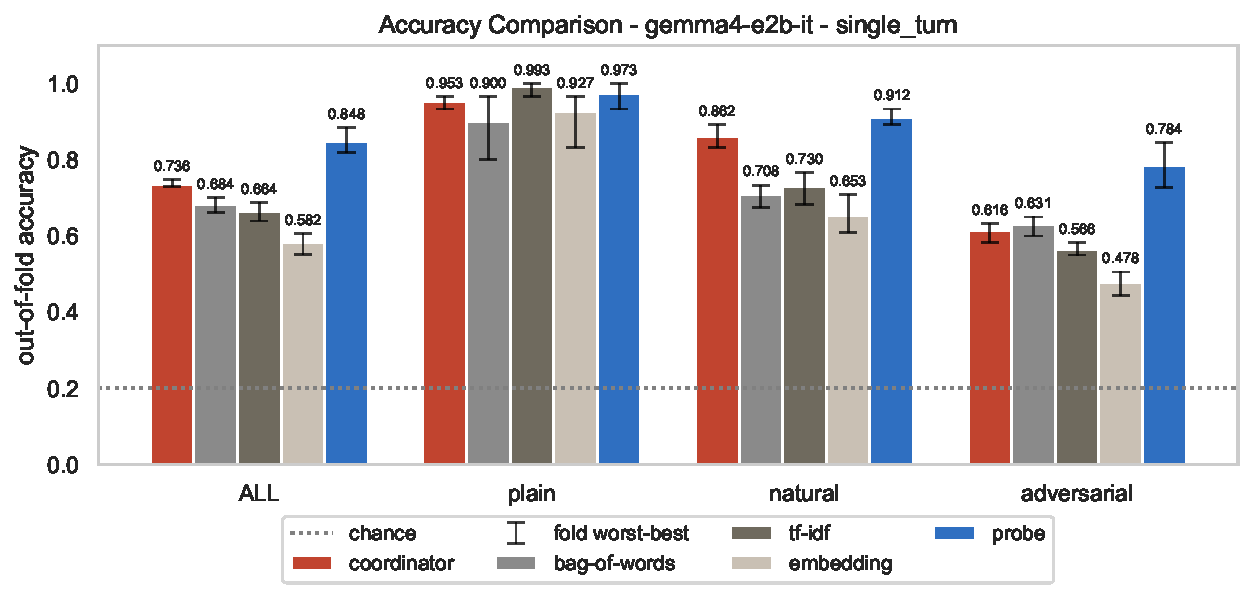
\includegraphics[width=0.85\textwidth]{images/models/gemma4-e2b-it_single_turn_routers.pdf}
    \caption[Accuracy comparison, gemma4-e2b-it, single-turn]{Accuracy comparison, gemma4-e2b-it, single-turn.}
    \label{fig:ch7-gemma4-e2b-it-single-routers}
\end{figure}

\begin{figure}[H]
    \centering
    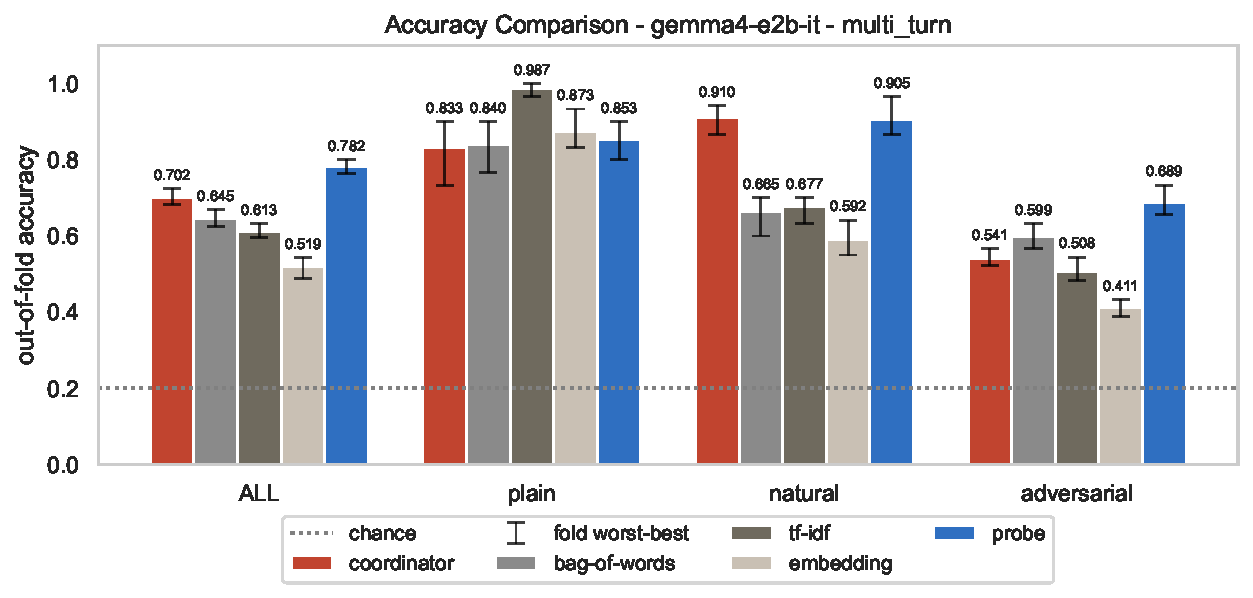
\includegraphics[width=0.85\textwidth]{images/models/gemma4-e2b-it_multi_turn_routers.pdf}
    \caption[Accuracy comparison, gemma4-e2b-it, multi-turn]{Accuracy comparison, gemma4-e2b-it, multi-turn.}
    \label{fig:ch7-gemma4-e2b-it-multi-routers}
\end{figure}


\clearpage

\subsection{Qwen3 4B Instruct 2507}
\label{subsec:ch7-qwen3-4b}

\begin{table}[H]
    \centering
    \small
    \setlength{\tabcolsep}{3.5pt}
    \begin{tabular}{@{}lcccccccccc@{}}
        \toprule
        & & & \multicolumn{4}{c}{\textbf{all}} & \multicolumn{4}{c}{\textbf{adversarial}} \\
        \cmidrule(lr){4-7} \cmidrule(lr){8-11}
        & \textbf{optimal layer} & \textbf{AUC macro} & \textbf{model} & \textbf{probe} & $\boldsymbol{\Delta}$ & $\boldsymbol{p_{\text{holm}}}$ & \textbf{model} & \textbf{probe} & $\boldsymbol{\Delta}$ & $\boldsymbol{p_{\text{holm}}}$ \\
        \midrule
        Single-turn & 23/36 & 0.977 & 0.752 & 0.864 & \rgain{0.112} & $<10^{-4}$ & 0.610 & 0.806 & \rgain{0.196} & $<10^{-4}$ \\
        Multi-turn & 23/36 & 0.959 & 0.745 & 0.814 & \rgain{0.069} & $<10^{-4}$ & 0.602 & 0.718 & \rgain{0.116} & $<10^{-4}$ \\
        \bottomrule
    \end{tabular}
    \caption[\texttt{qwen3-4b}, probe against model, both datasets]{\texttt{qwen3-4b}, probe against model, both datasets.}
    \label{tab:ch7-qwen3-4b}
\end{table}

\begin{figure}[H]
    \centering
    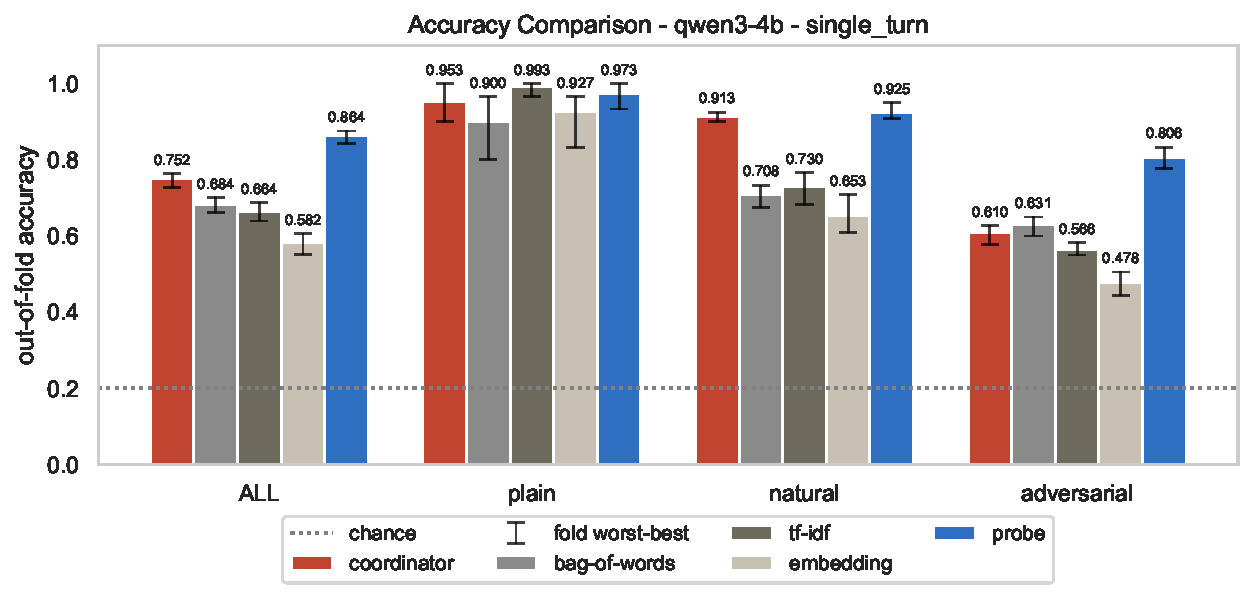
\includegraphics[width=0.85\textwidth]{images/models/qwen3-4b_single_turn_routers.pdf}
    \caption[Accuracy comparison, qwen3-4b, single-turn]{Accuracy comparison, qwen3-4b, single-turn.}
    \label{fig:ch7-qwen3-4b-single-routers}
\end{figure}

\begin{figure}[H]
    \centering
    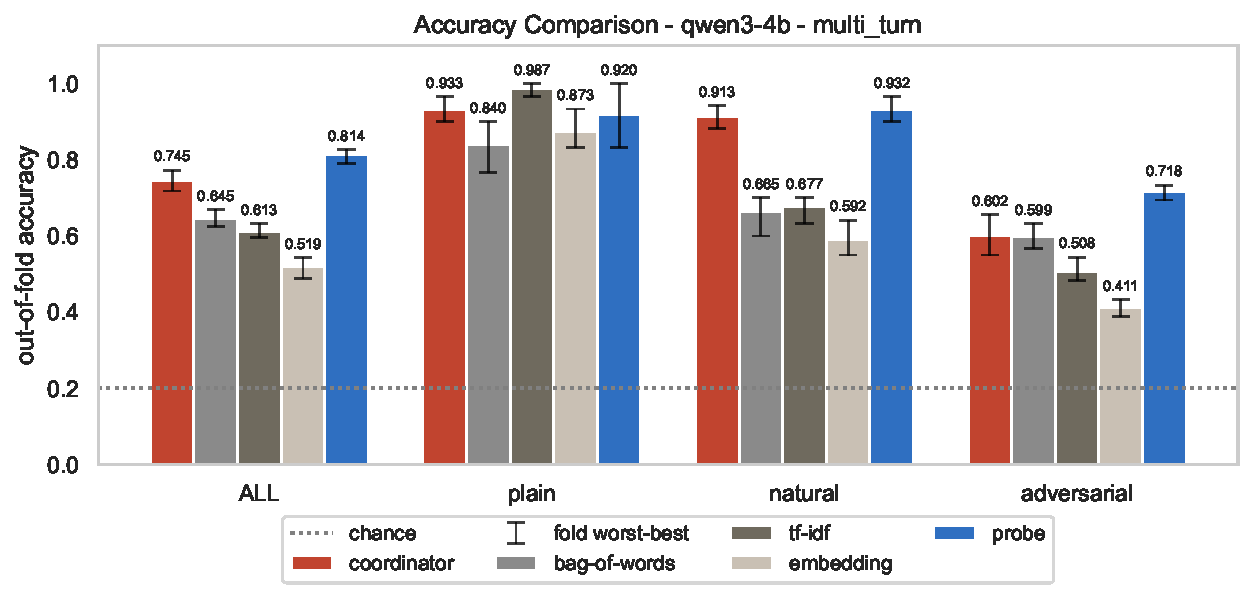
\includegraphics[width=0.85\textwidth]{images/models/qwen3-4b_multi_turn_routers.pdf}
    \caption[Accuracy comparison, qwen3-4b, multi-turn]{Accuracy comparison, qwen3-4b, multi-turn.}
    \label{fig:ch7-qwen3-4b-multi-routers}
\end{figure}


\clearpage

\subsection{Qwen3 8B}
\label{subsec:ch7-qwen3-8b}

\begin{table}[H]
    \centering
    \small
    \setlength{\tabcolsep}{3.5pt}
    \begin{tabular}{@{}lcccccccccc@{}}
        \toprule
        & & & \multicolumn{4}{c}{\textbf{all}} & \multicolumn{4}{c}{\textbf{adversarial}} \\
        \cmidrule(lr){4-7} \cmidrule(lr){8-11}
        & \textbf{optimal layer} & \textbf{AUC macro} & \textbf{model} & \textbf{probe} & $\boldsymbol{\Delta}$ & $\boldsymbol{p_{\text{holm}}}$ & \textbf{model} & \textbf{probe} & $\boldsymbol{\Delta}$ & $\boldsymbol{p_{\text{holm}}}$ \\
        \midrule
        Single-turn & 23/36 & 0.974 & 0.772 & 0.845 & \rgain{0.073} & $<10^{-4}$ & 0.652 & 0.784 & \rgain{0.132} & $<10^{-4}$ \\
        Multi-turn & 30/36 & 0.928 & 0.738 & 0.744 & \rgain{0.006} & \pns{0.65} & 0.597 & 0.634 & \rgain{0.037} & \pns{0.10} \\
        \bottomrule
    \end{tabular}
    \caption[\texttt{qwen3-8b}, probe against model, both datasets]{\texttt{qwen3-8b}, probe against model, both datasets.}
    \label{tab:ch7-qwen3-8b}
\end{table}

\begin{figure}[H]
    \centering
    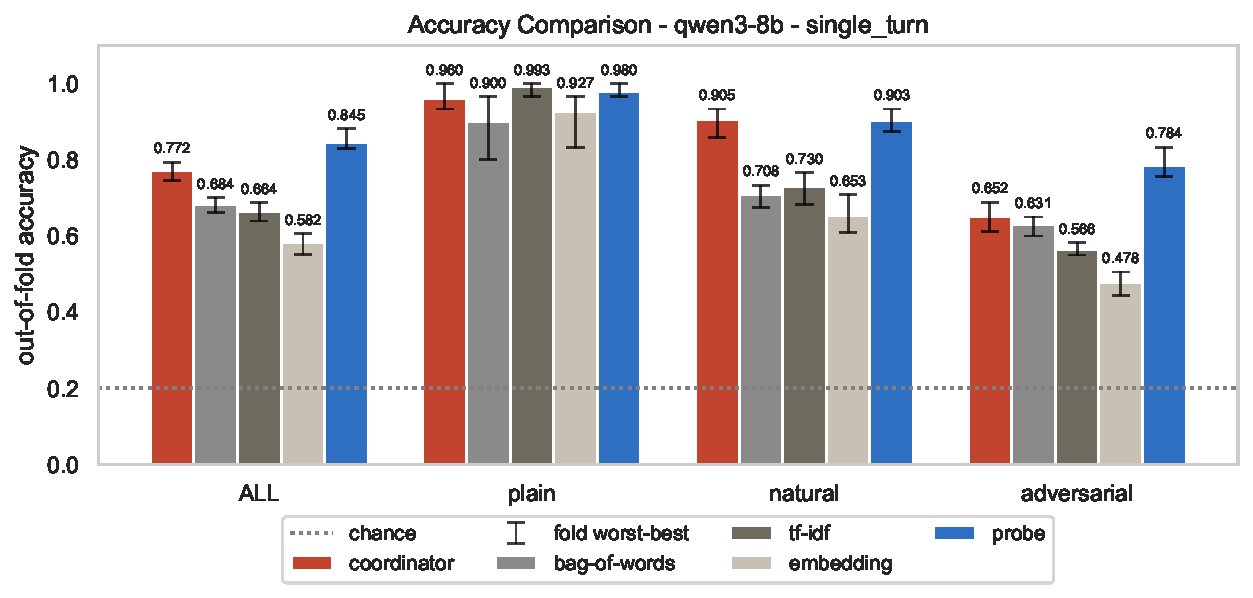
\includegraphics[width=0.85\textwidth]{images/models/qwen3-8b_single_turn_routers.pdf}
    \caption[Accuracy comparison, qwen3-8b, single-turn]{Accuracy comparison, qwen3-8b, single-turn.}
    \label{fig:ch7-qwen3-8b-single-routers}
\end{figure}

\begin{figure}[H]
    \centering
    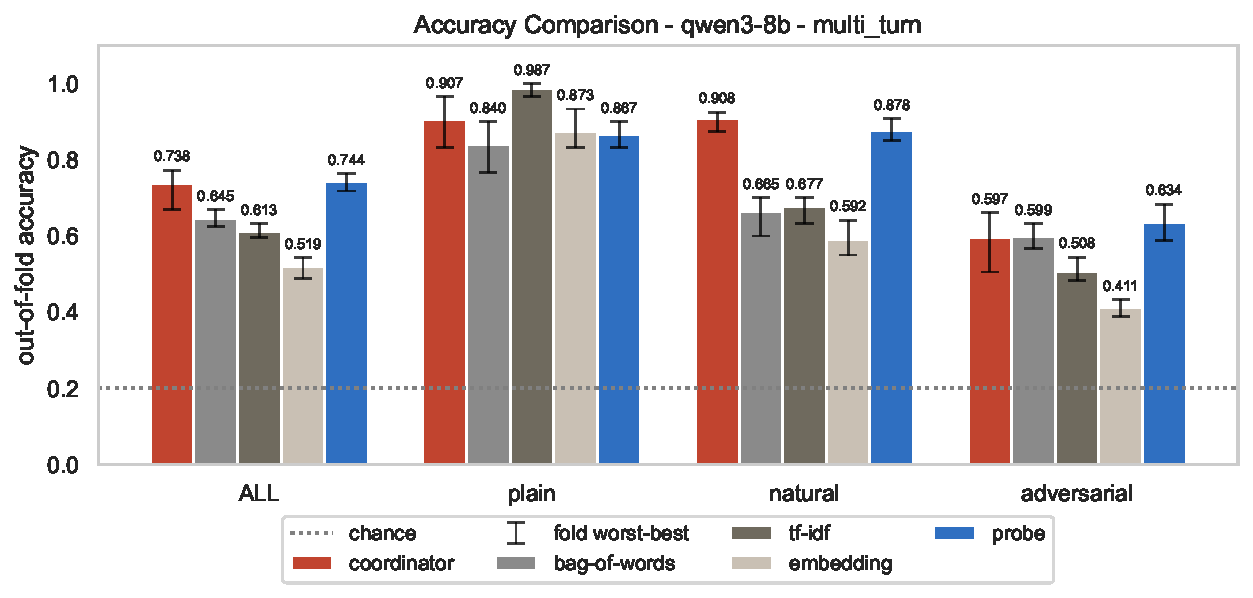
\includegraphics[width=0.85\textwidth]{images/models/qwen3-8b_multi_turn_routers.pdf}
    \caption[Accuracy comparison, qwen3-8b, multi-turn]{Accuracy comparison, qwen3-8b, multi-turn.}
    \label{fig:ch7-qwen3-8b-multi-routers}
\end{figure}


\clearpage

\subsection{Gemma 4 12B IT}
\label{subsec:ch7-gemma4-12b-it}

\begin{table}[H]
    \centering
    \small
    \setlength{\tabcolsep}{3.5pt}
    \begin{tabular}{@{}lcccccccccc@{}}
        \toprule
        & & & \multicolumn{4}{c}{\textbf{all}} & \multicolumn{4}{c}{\textbf{adversarial}} \\
        \cmidrule(lr){4-7} \cmidrule(lr){8-11}
        & \textbf{optimal layer} & \textbf{AUC macro} & \textbf{model} & \textbf{probe} & $\boldsymbol{\Delta}$ & $\boldsymbol{p_{\text{holm}}}$ & \textbf{model} & \textbf{probe} & $\boldsymbol{\Delta}$ & $\boldsymbol{p_{\text{holm}}}$ \\
        \midrule
        Single-turn & 31/48 & 0.988 & 0.873 & 0.916 & \rgain{0.043} & $<10^{-4}$ & 0.829 & 0.884 & \rgain{0.055} & $<10^{-4}$ \\
        Multi-turn & 32/48 & 0.979 & 0.855 & 0.879 & \rgain{0.024} & 0.011 & 0.777 & 0.827 & \rgain{0.050} & 0.00048 \\
        \bottomrule
    \end{tabular}
    \caption[\texttt{gemma4-12b-it}, probe against model, both datasets]{\texttt{gemma4-12b-it}, probe against model, both datasets.}
    \label{tab:ch7-gemma4-12b-it}
\end{table}

\begin{figure}[H]
    \centering
    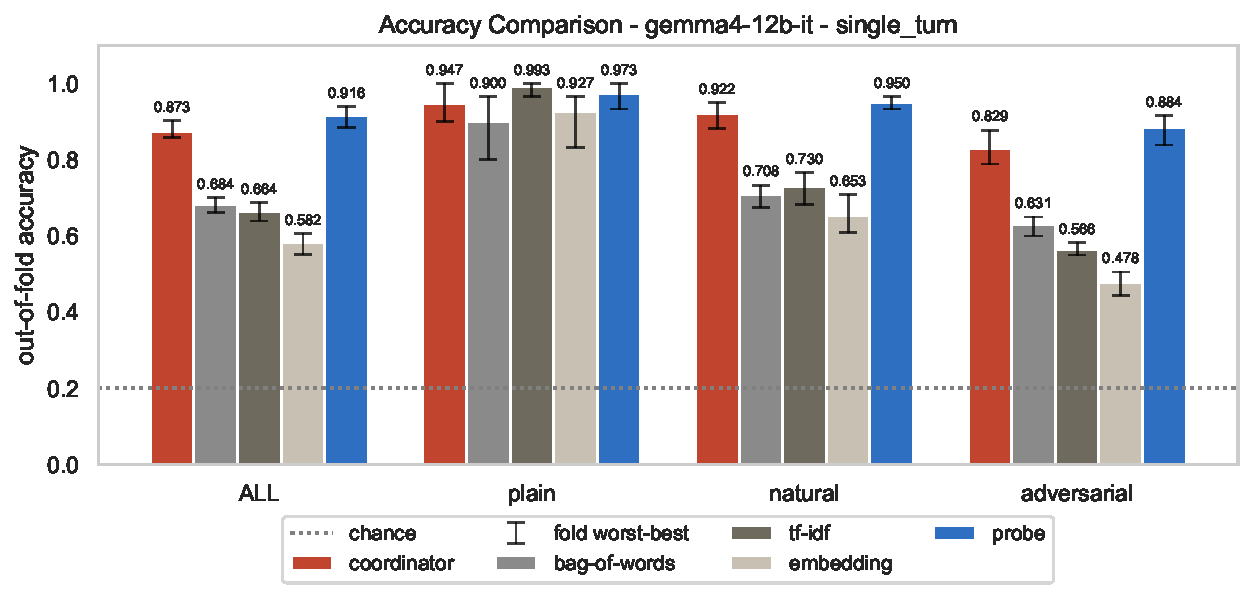
\includegraphics[width=0.85\textwidth]{images/models/gemma4-12b-it_single_turn_routers.pdf}
    \caption[Accuracy comparison, gemma4-12b-it, single-turn]{Accuracy comparison, gemma4-12b-it, single-turn.}
    \label{fig:ch7-gemma4-12b-it-single-routers}
\end{figure}

\begin{figure}[H]
    \centering
    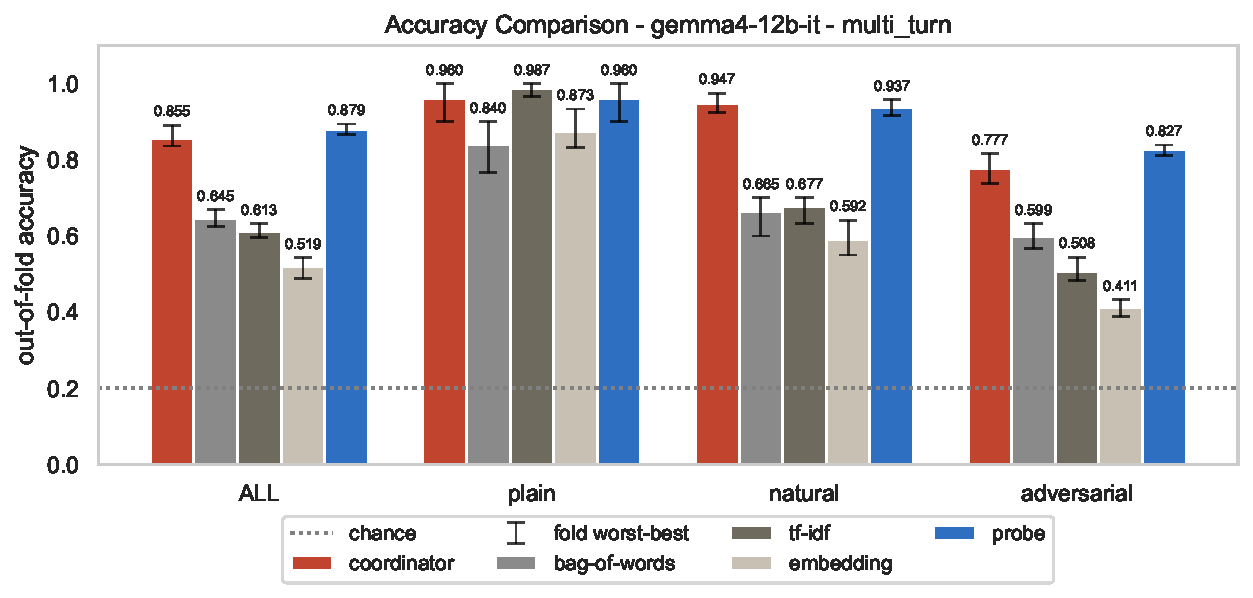
\includegraphics[width=0.85\textwidth]{images/models/gemma4-12b-it_multi_turn_routers.pdf}
    \caption[Accuracy comparison, gemma4-12b-it, multi-turn]{Accuracy comparison, gemma4-12b-it, multi-turn.}
    \label{fig:ch7-gemma4-12b-it-multi-routers}
\end{figure}


\clearpage

\subsection{GPT-OSS 20B}
\label{subsec:ch7-gpt-oss-20b}

\begin{table}[H]
    \centering
    \small
    \setlength{\tabcolsep}{3.5pt}
    \begin{tabular}{@{}lcccccccccc@{}}
        \toprule
        & & & \multicolumn{4}{c}{\textbf{all}} & \multicolumn{4}{c}{\textbf{adversarial}} \\
        \cmidrule(lr){4-7} \cmidrule(lr){8-11}
        & \textbf{optimal layer} & \textbf{AUC macro} & \textbf{model} & \textbf{probe} & $\boldsymbol{\Delta}$ & $\boldsymbol{p_{\text{holm}}}$ & \textbf{model} & \textbf{probe} & $\boldsymbol{\Delta}$ & $\boldsymbol{p_{\text{holm}}}$ \\
        \midrule
        Single-turn & 18/24 & 0.915 & 0.818 & 0.689 & \rgain{-0.129} & $<10^{-4}$ & 0.737 & 0.601 & \rgain{-0.136} & $<10^{-4}$ \\
        Multi-turn & 18/24 & 0.788 & 0.719 & 0.505 & \rgain{-0.214} & $<10^{-4}$ & 0.607 & 0.438 & \rgain{-0.169} & $<10^{-4}$ \\
        \bottomrule
    \end{tabular}
    \caption[\texttt{gpt-oss-20b}, probe against model, both datasets]{\texttt{gpt-oss-20b}, probe against model, both datasets.}
    \label{tab:ch7-gpt-oss-20b}
\end{table}

\begin{figure}[H]
    \centering
    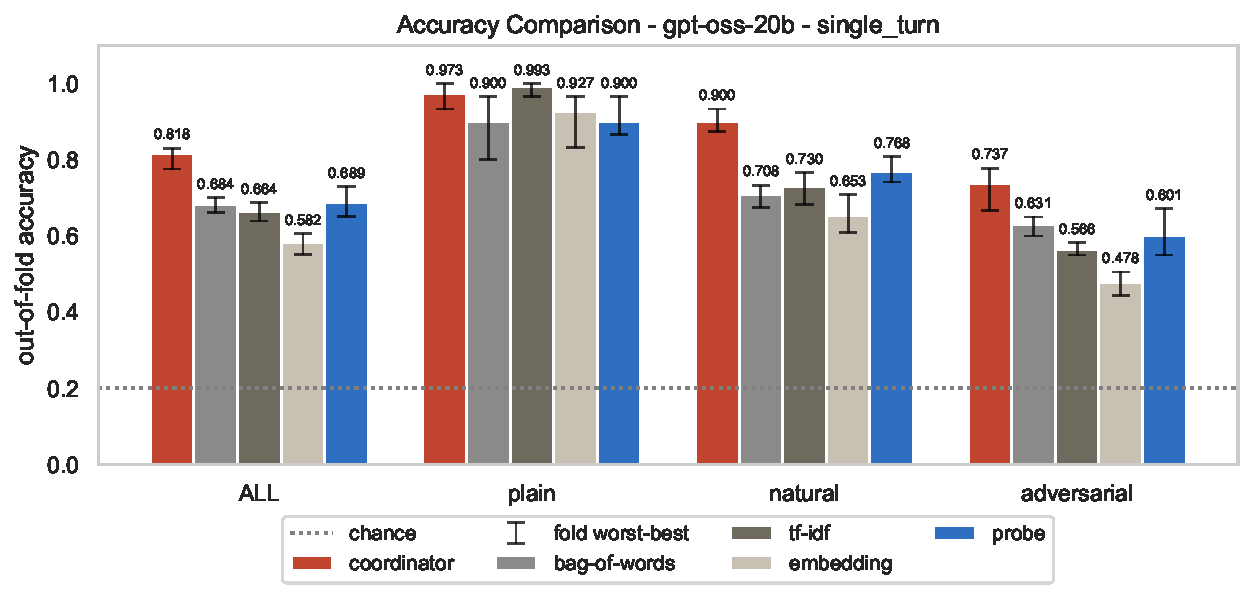
\includegraphics[width=0.85\textwidth]{images/models/gpt-oss-20b_single_turn_routers.pdf}
    \caption[Accuracy comparison, gpt-oss-20b, single-turn]{Accuracy comparison, gpt-oss-20b, single-turn.}
    \label{fig:ch7-gpt-oss-20b-single-routers}
\end{figure}

\begin{figure}[H]
    \centering
    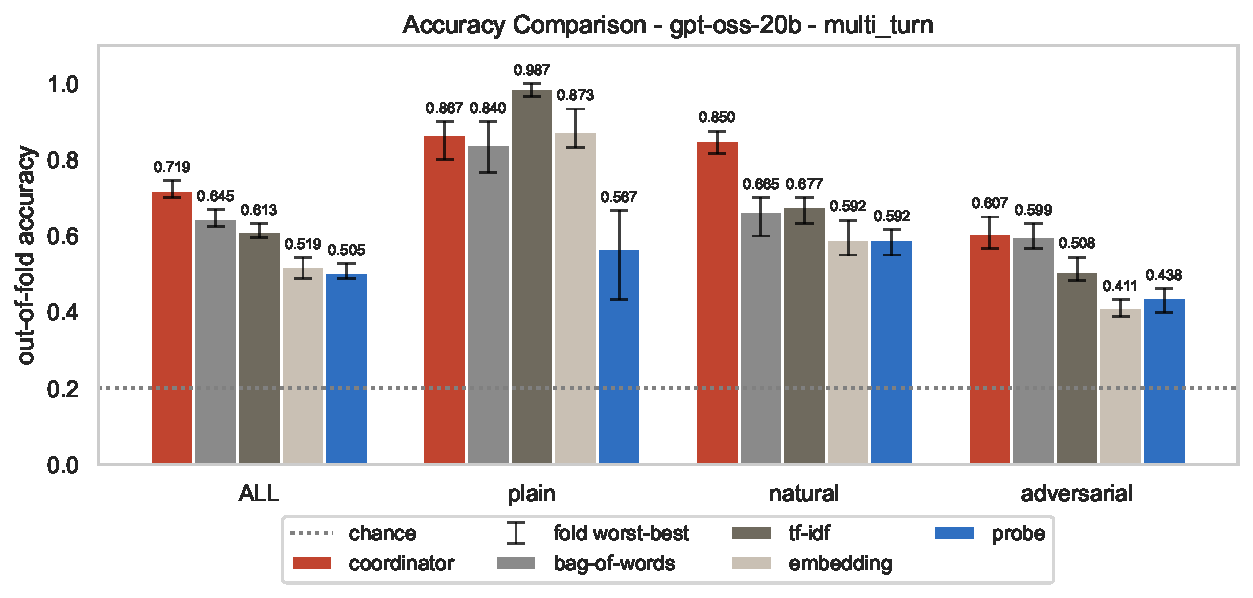
\includegraphics[width=0.85\textwidth]{images/models/gpt-oss-20b_multi_turn_routers.pdf}
    \caption[Accuracy comparison, gpt-oss-20b, multi-turn]{Accuracy comparison, gpt-oss-20b, multi-turn.}
    \label{fig:ch7-gpt-oss-20b-multi-routers}
\end{figure}


\clearpage

\subsection{Gemma 4 26B A4B IT}
\label{subsec:ch7-gemma4-26b-a4b-it}

\begin{table}[H]
    \centering
    \small
    \setlength{\tabcolsep}{3.5pt}
    \begin{tabular}{@{}lcccccccccc@{}}
        \toprule
        & & & \multicolumn{4}{c}{\textbf{all}} & \multicolumn{4}{c}{\textbf{adversarial}} \\
        \cmidrule(lr){4-7} \cmidrule(lr){8-11}
        & \textbf{optimal layer} & \textbf{AUC macro} & \textbf{model} & \textbf{probe} & $\boldsymbol{\Delta}$ & $\boldsymbol{p_{\text{holm}}}$ & \textbf{model} & \textbf{probe} & $\boldsymbol{\Delta}$ & $\boldsymbol{p_{\text{holm}}}$ \\
        \midrule
        Single-turn & 19/30 & 0.989 & 0.888 & 0.921 & \rgain{0.033} & 0.00012 & 0.841 & 0.888 & \rgain{0.047} & 0.001 \\
        Multi-turn & 19/30 & 0.977 & 0.856 & 0.878 & \rgain{0.022} & 0.024 & 0.773 & 0.831 & \rgain{0.058} & 0.00016 \\
        \bottomrule
    \end{tabular}
    \caption[\texttt{gemma4-26b-a4b-it}, probe against model, both datasets]{\texttt{gemma4-26b-a4b-it}, probe against model, both datasets.}
    \label{tab:ch7-gemma4-26b-a4b-it}
\end{table}

\begin{figure}[H]
    \centering
    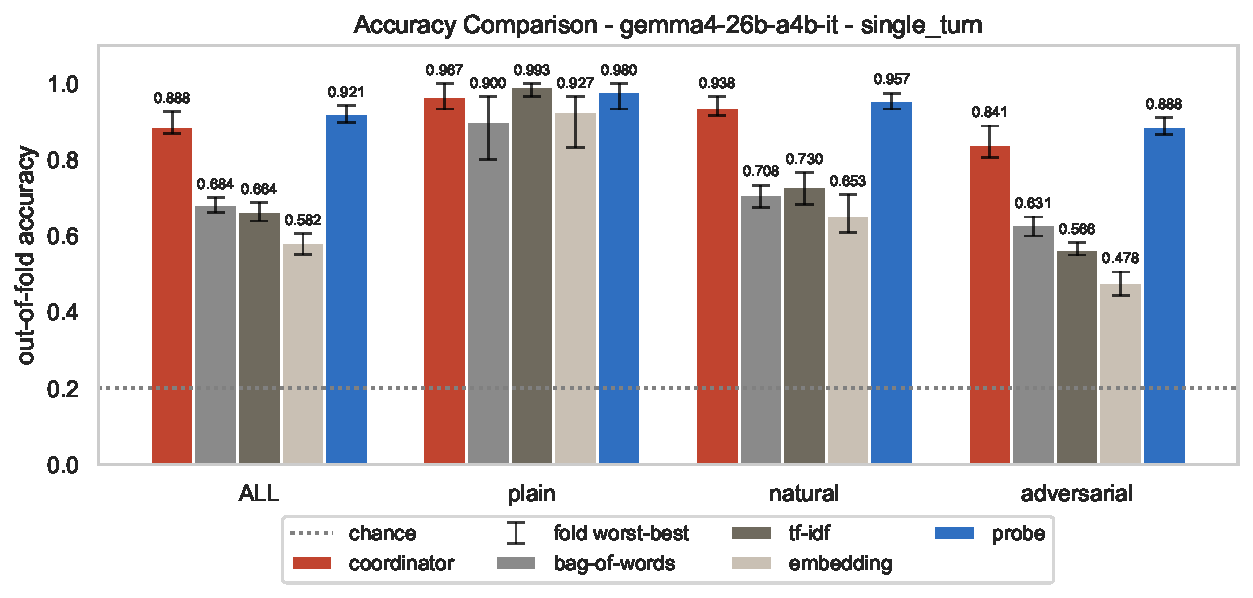
\includegraphics[width=0.85\textwidth]{images/models/gemma4-26b-a4b-it_single_turn_routers.pdf}
    \caption[Accuracy comparison, gemma4-26b-a4b-it, single-turn]{Accuracy comparison, gemma4-26b-a4b-it, single-turn.}
    \label{fig:ch7-gemma4-26b-a4b-it-single-routers}
\end{figure}

\begin{figure}[H]
    \centering
    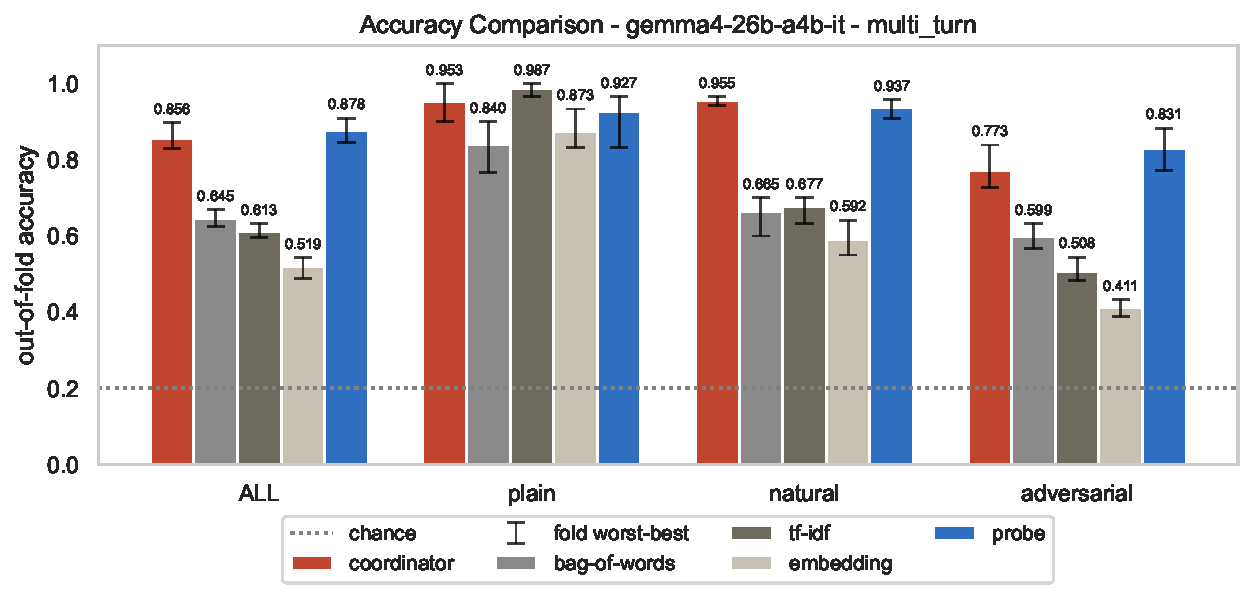
\includegraphics[width=0.85\textwidth]{images/models/gemma4-26b-a4b-it_multi_turn_routers.pdf}
    \caption[Accuracy comparison, gemma4-26b-a4b-it, multi-turn]{Accuracy comparison, gemma4-26b-a4b-it, multi-turn.}
    \label{fig:ch7-gemma4-26b-a4b-it-multi-routers}
\end{figure}


\clearpage

\subsection{Llama 3.3 70B Instruct}
\label{subsec:ch7-llama33-70b}

\begin{table}[H]
    \centering
    \small
    \setlength{\tabcolsep}{3.5pt}
    \begin{tabular}{@{}lcccccccccc@{}}
        \toprule
        & & & \multicolumn{4}{c}{\textbf{all}} & \multicolumn{4}{c}{\textbf{adversarial}} \\
        \cmidrule(lr){4-7} \cmidrule(lr){8-11}
        & \textbf{optimal layer} & \textbf{AUC macro} & \textbf{model} & \textbf{probe} & $\boldsymbol{\Delta}$ & $\boldsymbol{p_{\text{holm}}}$ & \textbf{model} & \textbf{probe} & $\boldsymbol{\Delta}$ & $\boldsymbol{p_{\text{holm}}}$ \\
        \midrule
        Single-turn & 42/80 & 0.985 & 0.770 & 0.894 & \rgain{0.124} & $<10^{-4}$ & 0.667 & 0.847 & \rgain{0.180} & $<10^{-4}$ \\
        Multi-turn & 38/80 & 0.950 & 0.736 & 0.810 & \rgain{0.074} & $<10^{-4}$ & 0.606 & 0.714 & \rgain{0.108} & $<10^{-4}$ \\
        \bottomrule
    \end{tabular}
    \caption[\texttt{llama3.3-70b}, probe against model, both datasets]{\texttt{llama3.3-70b}, probe against model, both datasets.}
    \label{tab:ch7-llama33-70b}
\end{table}

\begin{figure}[H]
    \centering
    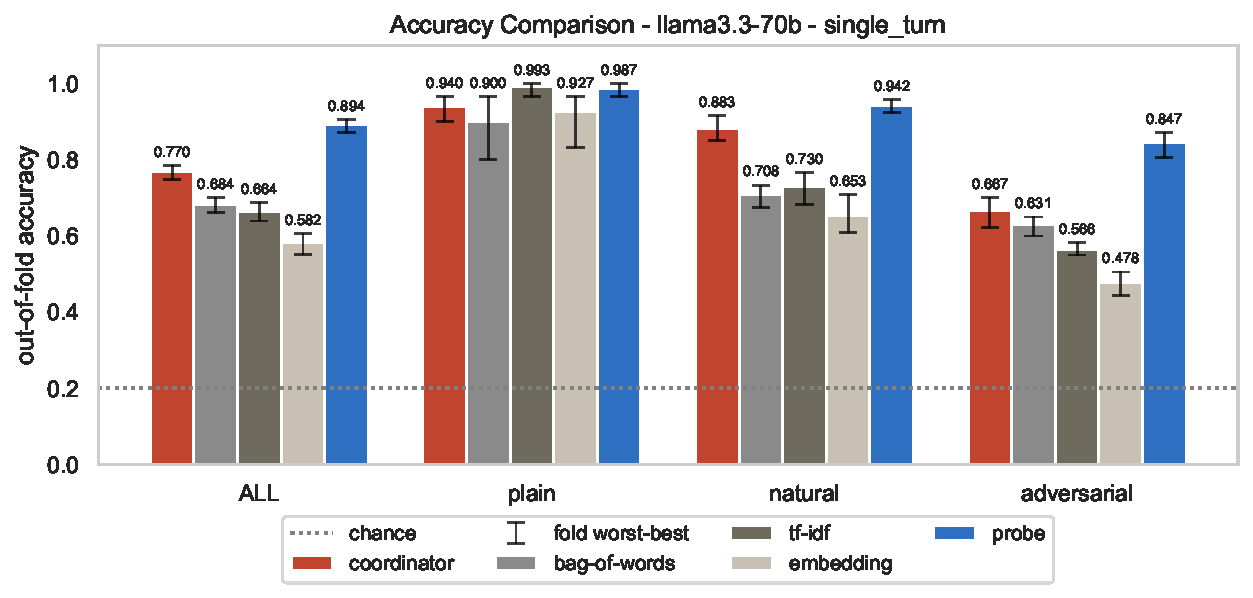
\includegraphics[width=0.85\textwidth]{images/models/llama33-70b_single_turn_routers.pdf}
    \caption[Accuracy comparison, llama3.3-70b, single-turn]{Accuracy comparison, llama3.3-70b, single-turn.}
    \label{fig:ch7-llama33-70b-single-routers}
\end{figure}

\begin{figure}[H]
    \centering
    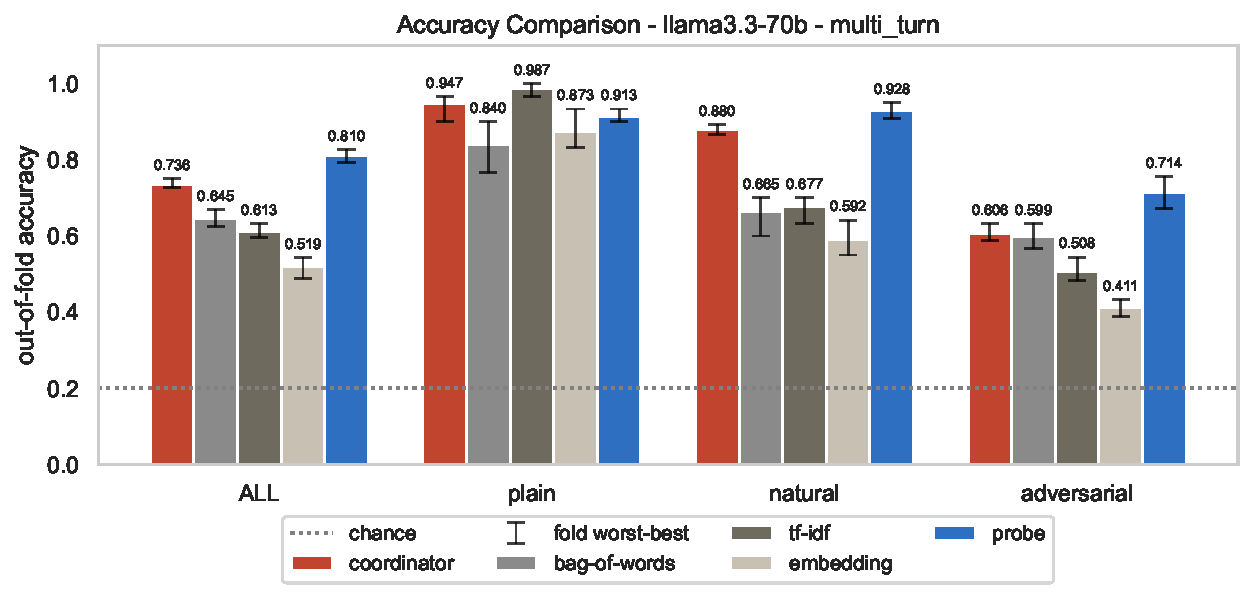
\includegraphics[width=0.85\textwidth]{images/models/llama33-70b_multi_turn_routers.pdf}
    \caption[Accuracy comparison, llama3.3-70b, multi-turn]{Accuracy comparison, llama3.3-70b, multi-turn.}
    \label{fig:ch7-llama33-70b-multi-routers}
\end{figure}


\clearpage

\subsection{Qwen2.5 72B Instruct}
\label{subsec:ch7-qwen25-72b}

\begin{table}[H]
    \centering
    \small
    \setlength{\tabcolsep}{3.5pt}
    \begin{tabular}{@{}lcccccccccc@{}}
        \toprule
        & & & \multicolumn{4}{c}{\textbf{all}} & \multicolumn{4}{c}{\textbf{adversarial}} \\
        \cmidrule(lr){4-7} \cmidrule(lr){8-11}
        & \textbf{optimal layer} & \textbf{AUC macro} & \textbf{model} & \textbf{probe} & $\boldsymbol{\Delta}$ & $\boldsymbol{p_{\text{holm}}}$ & \textbf{model} & \textbf{probe} & $\boldsymbol{\Delta}$ & $\boldsymbol{p_{\text{holm}}}$ \\
        \midrule
        Single-turn & 55/80 & 0.988 & 0.761 & 0.907 & \rgain{0.146} & $<10^{-4}$ & 0.638 & 0.862 & \rgain{0.224} & $<10^{-4}$ \\
        Multi-turn & 58/80 & 0.976 & 0.768 & 0.875 & \rgain{0.107} & $<10^{-4}$ & 0.629 & 0.800 & \rgain{0.171} & $<10^{-4}$ \\
        \bottomrule
    \end{tabular}
    \caption[\texttt{qwen2.5-72b}, probe against model, both datasets]{\texttt{qwen2.5-72b}, probe against model, both datasets.}
    \label{tab:ch7-qwen25-72b}
\end{table}

\begin{figure}[H]
    \centering
    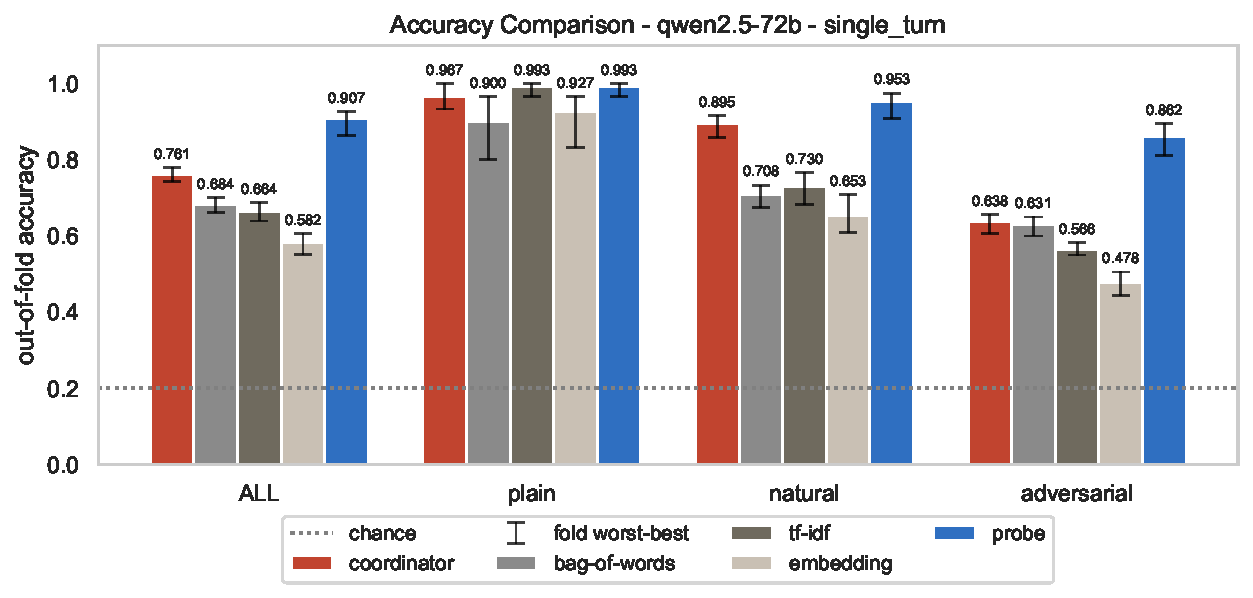
\includegraphics[width=0.85\textwidth]{images/models/qwen25-72b_single_turn_routers.pdf}
    \caption[Accuracy comparison, qwen2.5-72b, single-turn]{Accuracy comparison, qwen2.5-72b, single-turn.}
    \label{fig:ch7-qwen25-72b-single-routers}
\end{figure}

\begin{figure}[H]
    \centering
    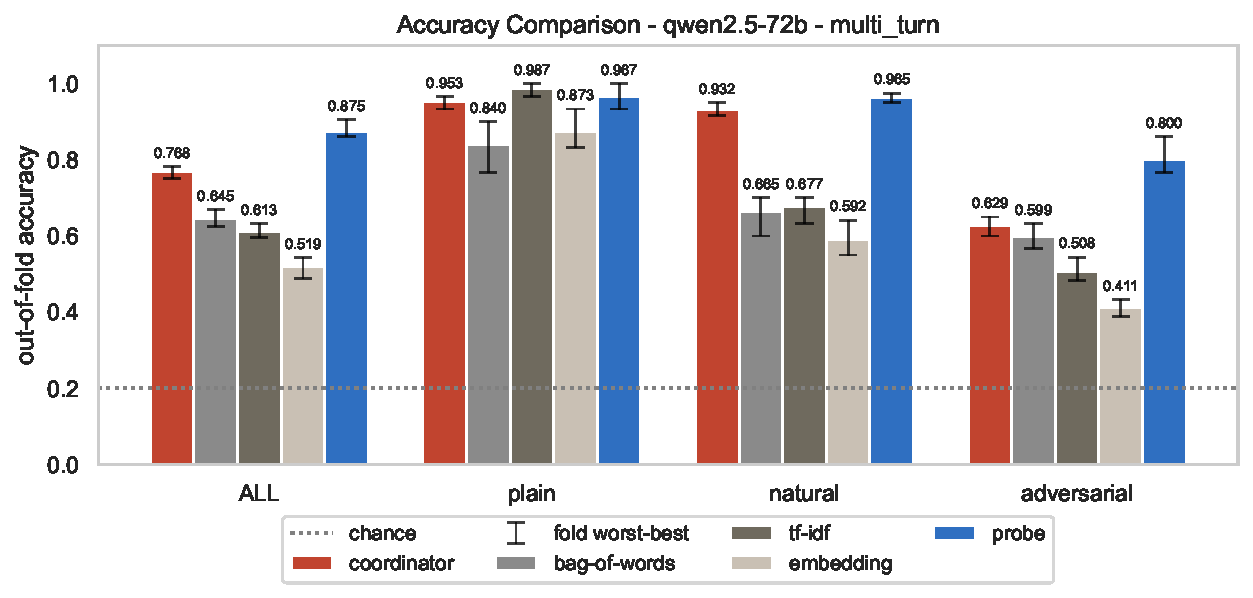
\includegraphics[width=0.85\textwidth]{images/models/qwen25-72b_multi_turn_routers.pdf}
    \caption[Accuracy comparison, qwen2.5-72b, multi-turn]{Accuracy comparison, qwen2.5-72b, multi-turn.}
    \label{fig:ch7-qwen25-72b-multi-routers}
\end{figure}



\clearpage
\section{Observations}
\label{sec:ch7-observations}

In all models except GPT-OSS 20B, the probe is more accurate than the model and than the three text-only classifiers, on both the whole single-turn and the whole multi-turn dataset. The difference between probe and model is significant according to the McNemar test, with one exception for Qwen3 8B on the whole multi-turn dataset ($p_{\text{holm}} = 0.65$). On the \texttt{plain} tier, the model, the probe and the text-only classifiers all score close to ceiling accuracy, and the TF-IDF classifier matches or exceeds the probe in every model. On the \texttt{natural} tier, the probe exceeds every text-only classifier by at least 0.17. On the single-turn dataset, it exceeds the model by 0.012 to 0.059 in six of the seven models, and it is 0.002 below the model for Qwen3 8B. On the \texttt{adversarial} tier, the accuracy of the probe exceeds the accuracy of every text-only classifier and of the model, on both datasets, and its difference from the model ranges from 0.037 to 0.224. This difference is significant in every model except Qwen3 8B on the multi-turn dataset ($p_{\text{holm}} = 0.10$). As the difficulty increases, the probe is the classifier that retains the most accuracy.

On the multi-turn dataset, the probe is less accurate than on the single-turn dataset in all eight models, and its AUC macro is also lower. This suggests that, in the multi-turn setting, the sub-agents are less clearly separable from the hidden states, making the classification harder for the probe. The model loses less accuracy between the two datasets, so the difference between probe and model is smaller on the multi-turn dataset.

GPT-OSS 20B, which is the third most accurate model on the single-turn dataset, is the exception to all the previous observations. Its probe is less accurate than its model on every tier of both datasets, and its AUC macro (0.915 single-turn, 0.788 multi-turn) is the lowest of the eight models. On the multi-turn dataset, its probe falls below the bag-of-words and the TF-IDF classifier on the whole dataset and on every tier. Among the eight models, GPT-OSS 20B is the only one whose reasoning cannot be disabled, so its routing decision may be formed after the last prompt token where the hidden states are probed.

Chapter~\ref{chap:results-analysis} analyzes these results in detail.

